\chapter{QR Code Structure and Generation}

This chapter describes the structural pattern of QR codes, and the encoding procedure which produce the QR code of the message. This part is dedicated to presentation of the the standard version, based on the ISO/IEC 18004-2006 standard \cite{1iso}. According to this standard, three inputs are considered. The first one is the message that should be encoded. The second input is the version of the QR-code which related to size of the QR-code matrix and amount of data for encoding. Finally the last input is the error correction level which is usually determined based on the application 


\section{General structure}

According to the ISO/IEC standard, the QR symbol consists of an array of square modules form a general big square shape. Similar to the representation of data, a dark black module is zero and a light module is one which leads to a black and white binary pattern. In three corners of the symbol which are top left, top right and bottom left, finder patterns are located preparing 360 degree pattern recognizing and reading of the QR-code. In addition, some range of sizes of symbols is provided. The smallest one is $21 \times 21$ modules (version 1) and the largest is  $177 \times 177$ (version 40). Generally the following formula describe the relationship between the number of version and the number of modules:
$$Modules_{Num} = 4 \times Version_{Num} + 17$$
 Four levels of Reed-Solomon error correction named as L,
M, Q and H are determined, providing the ability of recovering the $7\%$, $15\%$, $25\%$ and $30\%$ of the symbol codewords respectively. Next figure illustrates the structure
of a version 7 QR code \cite{1iso}.
\begin{figure}[h!]
  \caption{QR symbol of version 7 \cite{1iso}}
  \centering
    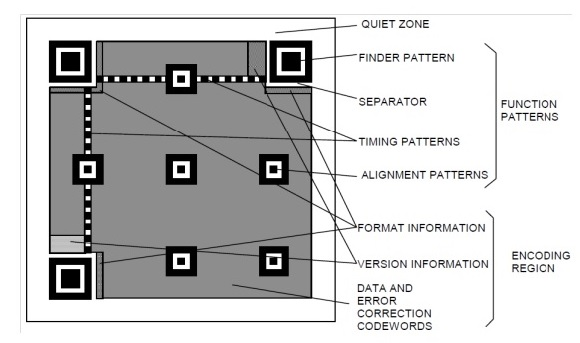
\includegraphics[width=1\textwidth]{figures/Figure21Version7QR.jpg}
    \label{fig:21}
\end{figure}

It is worth mentioning that the Figure \ref{fig:21} is a general format and is not necessary belongs to version 7. It can be present some other versions but it definitely demonstrates the general format of version 7 QR symbol. 

\section{Function Patterns}
"Encoding Regions" are related to the generation and decoding or QR symbol while "Function Patterns" are related to pattern recognition and scene understanding parts.\\
Function patterns are used for the Pattern Recognition and finding the location of the QR symbol and determining its
characteristics, in order to reconstruct the QR-Matrix for decoding process. Function patterns are not related to decoding message. QR-Matrix is simply consider a black module as 0 and a white module as 1. so the QR matrix of the version 1 is $21 \times 21$. More discussion about QR-Matrix would be provided in the subsequent sections Module positions form the QR-Matrix and defined by their row and column coordinates in the symbol, in the form (i, j) where i represents the row (top-down order) and j the column (left-right order) in which the module is located, with counting beginning at 1. Module (1, 1) is therefore located at the upper left corner of the symbol\cite{Thonky}.

\subsection{Finder Patterns}

There is only three \textbf{finder patterns} and are located at exactly three position of the symbol. The upper left, upper right and lower left corners of the symbol. Each finder pattern can be viewed as three concentric squares and is constructed of a black(dark) $7 \times 7$ modules, white(light) $5 \times 5$ modules and finally a dark $3 \times 3$ modules. The wideness ratio of alternative black and white module widths in each finder pattern is approximately 1:1:3:1:1 from any direction (the ratio might be exactly 1:1:3:1:1 depends on the view angle or direction.
This important characteristic help us two find the locations(locations of the centers) of the finder patterns. \textbf{The separator pattern} is a function pattern of all white(light) modules(It is a one module wide) that play the role of a border between the finder patterns and the data region of
the symbol.

\subsection{Alignment Patterns}

The alignment patterns are placed at some specific positions for each particular version, and allow the QR decoder to tolerate distortions when the code is distorted. Except for version 1, other versions have alignment patterns and the number of alignment pattern differ from version to version. Alignment patterns are similar to finder patterns Except for the ratio which is 1:1:1:1:1. The alignment patterns are placed in fixed positions that are defined in the standard \cite{1iso}.

\subsection{Timing Patterns}

The timing patterns are two alternating sequences of black and white modules determining module coordinates in the symbol. Their place is specific in the symbol; the horizontal timing pattern is along with the sixth row of the symbol
between the separators for the two upper finder patterns and the vertical timing pattern is along with the sixth column of the symbol between the separators of the top-left and bottom-left finder patterns. For better understanding, let's scan the sixth row(left to right) in the symbol which contains finder patters, separators and timing patterns. The first 7 modules are belong to top-left finder pattern. The 8th module is white which belongs to separator. Now let's scan this row from right to left. Again the first 7 modules are belong to right-left finder pattern. The 8th module is white which belongs to the other separator. Now the other modules in this row belongs to horizontal timing pattern which its length is:
$$Version*4+17-16=Version*4+1$$
Same procedure applied for vertical timing pattern and the lengths are the same.

\section{Encoding Region and Generating QR Symbol}\label{Encod}

If a region is not related to function patterns is related to data and is available for encoding and error correction, format and version information. The following subsections will explain the QR code encoding process in detail. Here is a general overview of the process which is necessary to understand before going through the encoding process\cite{Thonky}:

\textbf{Step 1: Data and Information Analysis}
The QR-Code generating process, encodes a message or in other word a sequence. There is four available modes for encoding text is QR standard: numeric, alphanumeric, byte, and Kanji. Each mode encodes the text as a sequence of bits (1s and 0s) which different method, and the goal is to produce the shortest possible sequence of bits. Consequently, the first step is to perform data analysis to determine which one of the four modes is optimal for your text.\\

\textbf{Step 2: Data Encoding}
After selecting the encoding mode, the next step is simply Encoding!! In the data encoding subsection this process is described is detail for each encoding mode. The result of this step is a sequence of bits that is split up into data codewords that are each 8 bits long.\\

\textbf{Step 3: Error Correction Coding}
QR codes use error correction in order to tolerate likely damages of image i.e. losing information. This means that after crating the sequence of data bits, error correction codewords should be generated using Reed-Solomon error correction. QR reading both the data codewords and the error correction codewords and comparing them, we're able to determine/correct errors.

\textbf{Step 4: Structure Final Message}
The generated data and error correction codewords, must be arranged in the appropriate order. For large QR codes, the data and error correction codewords are generated in blocks, and these blocks must be interleaved according to the QR code specification.\\

\textbf{Step 5: Module Placement in Matrix}
After generating the data codewords and error correction codewords and arranging them in the correct order, you must place the bits in the QR code matrix. The codewords are arranged in the matrix in a specific way. During this step, you will also place the patterns that are common to all QR codes, such as the boxes on the three corners.\\

\textbf{Step 6: Data Masking}
Certain patterns in the QR code matrix can make it difficult for QR code scanners to correctly read the code. To prevent this, the QR code specification defines eight mask patterns, each of which changes the QR code according to a particular pattern. You must determine which of these mask patterns results in the QR code with the fewest undesirable traits. This is done by evaluating each masked matrix based on four penalty rules. Your final QR code must use the mask pattern that resulted in the lowest penalty score.\\

\textbf{Step 7: Format and Version Information}
The final step is to add format and (if necessary) version information to the QR code by adding pixels in particular areas of the code that were left blank in previous steps. The format pixels identify the error correction level and mask pattern being used in this QR code. The version pixels encode the size of the QR matrix and are only used in larger QR codes.\\

\subsection{Data and Information Analysis}
The four encoding modes include the following characters:

\textbf{Numeric mode} is for decimal digits 0 through 9.

\textbf{Alphanumeric mode} is for the decimal digits 0 through 9, as well as uppercase letters (not lowercase!), and the symbols $\$, \%, *, +, -, ., /,$ and : as well as a space.

\textbf{Byte mode}, by default, is for characters from the ISO-8859-1 character set.

\textbf{Kanji mode} is for double-byte characters from the Shift JIS character set. While UTF-8 can encode Kanji characters, it must use three or four bytes to do so. Shift JIS, on the other hand, uses just two bytes to encode each Kanji character, so Kanji mode compresses Kanji characters more efficiently. If the entire input string consists of characters in the double-byte range of Shift JIS, use Kanji mode. It is also possible to use multiple modes within the same QR code.

\subsubsection{How to Choose the Most Efficient Mode}

To select the most efficient mode for the QR code, The characters in the input string and the following conditions should be checked:

If the input string only consists of decimal digits (0 through 9), use numeric mode.\\

If numeric mode is not applicable, and if all of the characters in the input string can be found in the alphanumeric table, use alphanumeric mode. \emph{letters CANNOT be encoded in alphanumeric mode; only uppercase.}\\

If there is a character that is not in the alphanumeric table but can be encoded in ISO 8859-1, use byte mode. As mentioned above, QR code readers may be able to recognize UTF-8 in byte mode.\\


\subsection{Data Encoding}
Each encoding mode is aimed to create the string of bits for the characters that are used in the specific mode. Each mode uses a different method for encoding data into bits.

\subsubsection*{Step 1: Choose the Error Correction Level} 

Before encoding the data, an error correction level should be chosen. QR codes use Reed-Solomon error correction. This process creates error correction codewords based on the encoded data. Error correction is determined for first detecting the error and second correcting it. Since Reed-Solomon coding is a symmetric coding, the error correction codewords simply will be followed by the data codewords. There are four levels of error correction: L, M, Q, H. Table \ref{table2.1} demonstrates the levels and their corresponding error correction capabilities:

\begin{table}[h!]
  \centering
          \caption{Error Correction Table}
         \label{table2.1}
    \begin{tabular}{| l | l |}
    \hline
    Error Correction Level & Error Correction Capability \\ \hline
    L & 7\% data recovery  \\ \hline
    M & 15\% data recovery  \\ \hline
    Q & 25\% data recovery \\ \hline
    H & 30\% data recovery \\ \hline
    \end{tabular}

\end{table}

Error correction penalize the system design and rate which means that it increase the complexity and the number of required bits.

\subsubsection*{Step 2: Determine the Smallest Version for the Data}

As we described before, the different sizes of QR codes are called versions. Each version is 4 pixels larger than the previous version. Each version has a maximum capacity, depending on the mode in use. In addition, the error correction level further restricts the capacity . The character capacities table lists \cite{1iso} the capacities of all QR versions for a given encoding mode and error correction level.

\textbf{How to Determine the Smallest Version}\\
At this point, count the number of characters to be encoded, and determine which is the smallest version that can contain that number of characters for the encoding mode and desired error correction level.

For example, the phrase "HELLO WORLD" has 11 characters. If encoding it with level Q error correction, since a version 1 code using level Q error correction can only contain 10 characters in alphanumeric mode\footnote{According to the character capacities table}, Therefore, the smallest version that can be used in this case is version 2.

\subsubsection*{Step 3: Add the Mode Indicator}


The encoded data must start with the corresponding mode indicator that specifies the mode being used for the subsequent bits that come after it. Table \ref{table2.2} lists the mode indicators for each mode. For example, Since encoding "HELLO WORLD" in alphanumeric mode, the encoded data must start with 0010.

\begin{table}[h!]
  \centering
          \caption{Mode Indicator Table}
         \label{table2.2}
    \begin{tabular}{| l | l |}
    \hline
    Mode name & Mode indicator \\ \hline
    Numeric Mode & 0001  \\ \hline
    Alphanumeric Mode & 0010  \\ \hline
    Byte Mode & 0100  \\ \hline
    Kanji Mode & 1000  \\ \hline
    \end{tabular}

\end{table}

\subsubsection*{Step 4: Add the Character Count Indicator}

\emph{The character count indicator is a sequence of bits that shows the number of characters that are being encoded}. The character count indicator must be placed after the mode indicator. Furthermore, the character count indicator must be a certain number of bits long, depending on the QR version.

Count the number of characters in the original input text, then convert that number into binary. The length of the character count indicator depends on the encoding mode and the QR code version that will be in use. To make the binary string the appropriate length, we need to zero-padding at the left.

The following lists contain the sizes of the character count indicators for each mode and version. For example, if encoding "HELLO WORLD" in a version 1 QR code in alphanumeric mode, the character count indicator must be 9 bits long. The character count of HELLO WORLD is 11. In binary, 11 is 1011. Pad it on the left to make it 9 bits long: 000001011. Put this after the mode indicator from step 3 to get the following bit string: 0010 000001011

\textbf{Versions 1 through 9}\\
Numeric mode: 10 bits\\
Alphanumeric mode: 9 bits\\
Byte mode: 8 bits\\
Japanese mode: 8 bits\\
\textbf{Versions 10 through 26}\\
Numeric mode: 12 bits\\
Alphanumeric mode: 11 bits\\
Byte mode: 16\\
Japanese mode: 10 bits\\
\textbf{Versions 27 through 40}\\
Numeric mode: 14 bits\\
Alphanumeric mode: 13 bits\\
Byte mode: 16 bits\\
Japanese mode: 12 bits\\

Since we only consider version 1 through 6 in this project, the numbers for version 1 through 9 would applied.

\subsubsection*{Step 5: Encode Using the Selected Mode}

The previous section, data analysis, explains how to select the appropriate encoding mode for a given string. The process for each encoding mode is explained in\cite{Thonky}.

\subsubsection*{Step 6: Break Up into 8-bit Codewords and Add Pad Bytes if Necessary}


After obtaining a string of bits that consists of the mode indicator, the character count indicator, and the data bits as described in steps 1 through 3, it may be necessary to add 0s and pad bytes, because the QR code standard specification requires that the bit string must completely fill the total capacity of the QR code.

\textbf{Determine the Required Number of Bits for this QR Code}\\
To determine how many data bits are required for a particular QR code, refer to the \cite{1iso}. Find the version and error correction level that is in use for the QR code being encoded, and find the number in the column that is labeled "Total Number of Data Codewords for this Version and EC Level". Multiply this number by 8 to obtain the total number of data bits required for this version and error correction level.

For example, according to the table, a version 1-Q code has 13 total data codewords. Therefore, the total number of bits required for this QR code is 13 * 8, or 104 bits.

\textbf{Add a Terminator of 0s if Necessary}\\
If the bit string is shorter than the total number of required bits, a terminator of up to four 0s must be added to the right side of the string. If the bit string is more than four bits shorter than the required number of bits, add four 0s to the end. If the bit string is fewer than four bits shorter, add only the number of 0s that are needed to reach the required number of bits.

For example, if encoding HELLO WORLD in a version 1-Q QR code, the total number of required bits is 104 bits. The data bit string is 74 bits long. The terminator must only be at most 4 bits long, so add four 0s to the right of the string. The resulting string is still too short to fill the 104 bit capacity, but the QR code specification requires that the terminator be at most four 0s in length. If the string had been 102 bits instead, the terminator would only be 2 bits in length.

\textbf{Add More 0s to Make the Length a Multiple of 8}\\
After adding the terminator, if the number of bits in the string is not a multiple of 8, first pad the string on the right with 0s to make the string's length a multiple of 8.

For example, after adding the terminator to the HELLO WORLD string, the length became 78 bits long. This is not a multiple of 8. The bit string is shown here broken up into 8-bit binary bytes:
00100000 01011011 00001011 01111000 11010001 01110010 11011100 01001101 01000011 010000

There are six bits at the end. Add two 0s to make it an 8-bit binary byte:

00100000 01011011 00001011 01111000 11010001 01110010 11011100\\ 01001101 01000011 010000\textbf{00}

\textbf{Add Pad Bytes if the String is Still too Short}\\
If the string is still not long enough to fill the maximum capacity, add the following bytes to the end of the string, repeating until the string has reached the maximum length:
11101100 00010001

These bytes are equivalent to 236 and 17, respectively. They are specifically required by the QR code specification to be added if the bit string is too short at this stage.

For example, the HELLO WORLD string above is 80 bits long. The required capacity for a 1-Q code, as stated earlier on the page, is 104 bits. The number of bits that must be added to fill the remaining capacity is 104 - 80, or 24. Divide this by 8: 24 /8 = 3. Therefore, three pad bytes must be added to the end of the data string. This is shown below:
00100000 01011011 00001011 01111000 11010001 01110010 11011100\\ 01001101 01000011 01000000 \textbf{11101100 00010001 11101100}

\subsection{Error Correction Coding}

Error correction coding provides appropriate conditions to extract the correct bit stream and decode the QR-code message in noisy scenarios. In other words if the image is corrupted or blur we may loss information by not correctly detecting the bits. In other scenario some parts of the QR pattern might be unavailable by any reason. The task of error correction decoding is to detect and correct the errors. Reed-Solomon coding is used for QR-code generation. After performing the previous part and transforming each 8-bits to a decimal number, we have decimal sequence. In this part according to this decimal sequence an error correction sequence has to be generated. This error correction sequence is added to the data codewords and they both form another longer decimal sequence. The length of error correction codewords depends on three factors:
\begin{itemize}
\item Length of data sequence
\item Version of QR code
\item Error correction level
\end{itemize}

Remember that in some cases( Different versions and error correction levels) the data would be broken to different sub-blocks and for each of sub-block a unique error correction sequence would be generated. Finally the data and error correction sequences will be interleaved in some specific order\cite{1iso}.

\subsection{Structure Final message}

In this part the interleaved data and error correction level is ready to form the final message. The decimal sequence now should be transformed to a binary sequence which obviously its length is a multiple of 8. The problem is the QR-Matrix should be fulled. Lots of QR matrices in different version doesn't have 8-divisible module numbers. \emph{So in version 2 through 7 the standard required that 7 reminder bits be added to the end of the generated bit stream}. For version 1 there is no need for any reminder bits.

\subsection{Module Placement in Matrix}

Suppose that after previous steps, Now we have the binary message which we need to put in the QR format. Some consideration are worth to consider. This part dedicated to the method and procedure for placing bit stream into the QR code\cite{Thonky}.

\subsubsection{Review of Function Patterns}

QR codes must include function patterns. These are shapes that must be placed in specific areas of the QR code to ensure that QR code scanners can correctly identify and orient the code for decoding. Figure \ref{fig:22} gives an example of what the function patterns are and where they are positioned. The finder patterns are the three blocks in the corners of the QR code at the top left, top right, and bottom left.

\textbf{The separators} are areas of white-space beside the finder patterns.

\textbf{The alignment patterns} are similar to finder patterns, but smaller, and are placed throughout the code. They are used in versions 2 and larger, and their positions depend on the QR code version.

\textbf{The timing patterns} are dotted lines that connect the finder patterns.

\textbf{The dark module} is a single black module that is always placed beside the bottom left finder pattern.

The sections below explain in greater detail how to position the function patterns. 
\begin{figure}[H]
  \caption{QR symbol\cite{Thonky}}
  \centering
    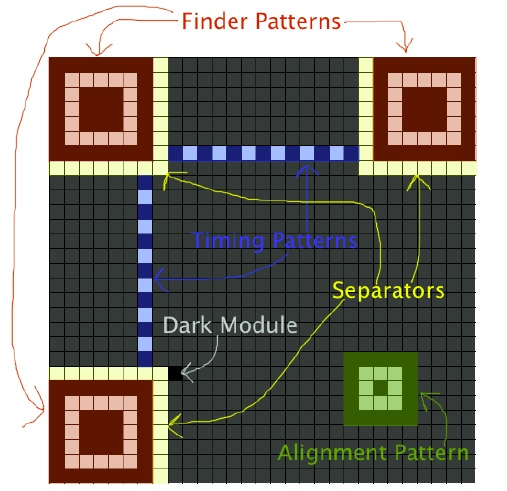
\includegraphics[width=0.4\textwidth]{figures/QR.jpg}
    \label{fig:22}
\end{figure}

Remember that we only consider version 1 through 6 for explaining these parts but also remember that the majority of explanations are the same for higher versions.\\
\\
\subsubsection{Finder Patterns}

 Any finder pattern consists of a square that is 7 modules by 7 modules, an inner white square that is 5 modules by 5 modules, and a full black square in the center that is 3 modules by 3 modules. The finder pattern is a special pattern which is almost impossible to be find in the other parts of the QR-code which is shown is Figure \ref{fig:23}. The module of the finder pattern have a ratio of 1:1:3:1:1. This ration is for alternative black and white modules which stats with black and obviously end by black again.
 
 \begin{figure}[H]
  \caption{Finder Pattern}
  \centering
    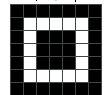
\includegraphics[width=0.3\textwidth]{figures/Finderpattern.jpg}
    \label{fig:23}
\end{figure}

In all versions the finder patterns are placed in the top left, top right, and bottom left corners of the QR code. The finder pattern can be find by the center of its inner solid black square. here are the centers for different finder patterns(first number in the bracket is row and second one is column):

\begin{itemize}
\item \textbf{top-left:} $[4,4]$
\item \textbf{top-right:} $[4,(4*version+17)-3]$
\item \textbf{down-left:} $[(4*version+17)-3,4]$
\end{itemize}

\subsubsection{Separators}

The separators are exactly separator lines of white modules(One module wide) that are placed beside the finder patterns to isolate them from the other of the QR code. The separators are only placed beside the edges of the finder patterns that touch the inside of the QR code. Consider the rounding area of the top-left finder pattern: 
\begin{figure}[H]
  \caption{Separator}
  \centering
    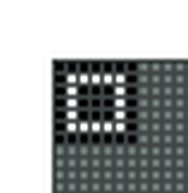
\includegraphics[width=0.3\textwidth]{figures/Separator.jpg}
    \label{fig:24}
\end{figure}


\subsubsection{Alignment Pattern}

QR codes that are version 2 and larger are required to have alignment patterns. An alignment pattern is similar to the finder pattern by the difference in the center square which is only a $1\times1$ black module rather then and $3\times3$ black square.

In version 1 through 6 the alignment patter(its center which is the dark black module) is placed at the $[(4*version+17)-6,(4*version+17)-6]$. As it is obvious from Figure \ref{fig:25} the center of Alignment Pattern is exactly in the column which the left-most black modules of the top-right finder patter exists and also in the row of which the most top black modules of the down-left finder patter exists.
\begin{figure}[H]
  \caption{Alignment Pattern}
  \centering
    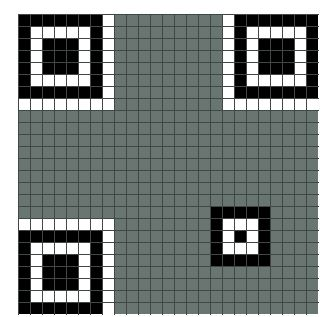
\includegraphics[width=0.3\textwidth]{figures/Alignmentpattern.jpg}
    \label{fig:25}
\end{figure}

\subsubsection{Timing Patterns}

The timing patterns are two horizontal and vertical lines of alternating dark and light modules. The horizontal and vertical timing patterns are placed on the 6th row and 6th column of the QR code respectively between the separators. The timing patterns always start and end with a dark module otherwise it's hard to
realize the starting point of the timing pattern because the separator is white. Figure \ref{fig:26} images show timing patterns on versions 2 through 6.

\begin{figure}[H]
  \caption{Timing Patterns}
  \centering
    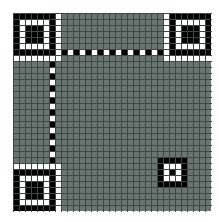
\includegraphics[width=0.5\textwidth]{figures/Timingpattern.jpg}
    \label{fig:26}
\end{figure}

\subsubsection{Dark Module and Reserved Areas}

Before adding the data bits to the QR code matrix, the dark module must be added, and there are areas of the matrix that must be reserved for the format and version bits, which will be added later. All QR codes have a dark module located at the coordinate $([(4 * Version) + 9], 8)$ where V is the version of the QR code. A strip of modules in neighborhoods of the separators must be reserved for the format information area as follows:
\begin{itemize}
\item Near the top-left finder pattern, a one-module strip must be reserved below and to the right of the separator.
\item Near the top-right finder pattern, a one-module strip must be reserved below the separator.
\item Near the bottom-left finder pattern, a one-module strip must be reserved to the right of the separator.
\end{itemize}


Figure \ref{fig:27} demonstrates the framework.
\begin{figure}[H]
  \caption{Reserved Area\cite{Thonky}}
  \centering
    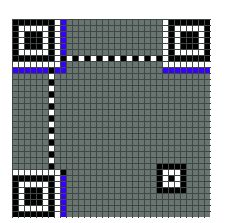
\includegraphics[width=0.5\textwidth]{figures/ReservedArea.jpg}
    \label{fig:27}
\end{figure}

\subsubsection{Placing the Data Bits}

Now we have the data bits and we want to place it in the matrix. Except for the aforementioned function patterns, dark module and reserved area other QR-Matrix entries should be filled with the bit stream which was produced by the data encoding part.
For filling the matrix there is a pattern. 

The data bits are placed beginning at the bottom-right of the matrix and continuing upward in a column that is 2-modules wide. When the column reaches the top, the next 2-module column starts to the left of the previous column and continues downward. Whenever the current column reaches the edge of the matrix, move on to the next 2-module column and reverse direction. If a function pattern or reserved area is reached, the data bit is placed in the next unused module.

The following figure demonstrates this pattern:
Figure \ref{fig:27} demonstrates the framework.
\begin{figure}[H]
  \caption{QR-Matrix Bit Allocating Pattern\cite{Thonky}}
  \centering
    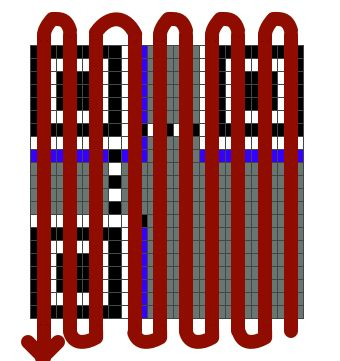
\includegraphics[width=0.5\textwidth]{figures/Feeding.jpg}
    \label{fig:28}
\end{figure}

In the Figure \ref{fig:28} in any 2-module length column there is a pattern for fulfilling the matrix places which is demonstrated in Figure \ref{fig29}.
%%%%%%%%%%%%%%%%
%%%%%%%%%%%%%%%%%%%%%%%%%%%%%%%%%%%%%%%%%
\begin{figure}[ht!]
     \begin{center}
%
        \subfigure[Upward bit allocating]{%
            \label{fig:first}
            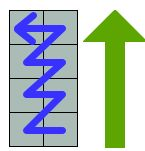
\includegraphics[width=0.4\textwidth]{figures/upwardfeed.jpg}
        }%
        \subfigure[Downward bit allocating]{%
           \label{fig:second}
           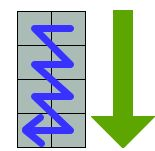
\includegraphics[width=0.4\textwidth]{figures/downwardfeed.jpg}
        }%  ------- End of the first row 
    \end{center}
    \caption{%
The inner pattern for upward and downward bit allocation\cite{Thonky}
     }%
   \label{fig29}
\end{figure}
%%%%%%%%%%%%%%%%%%%%%%%%%%%%%%%%%%%%%%%%%%%%%%%%
%%%%%%%%%%%%%%%%%%%%%%%%%%%%%%%%%%%%%%%%%%%

\subsection{Data Masking}

After placing the bit stream in the QR-Matrix, Now a mask pattern must be applied to the data part in the matrix. Remember that function patterns and other reserved area are not included in the masking procedure. The process of data masking change dark modules to bright and reverse in some specific way. 

There is 8 different mask patterns. Each of them should be applied to the matrix and for any of them a penalty score should be calculated\cite{1iso}. Any of the mask patterns which provides less penalty score is the most appropriate one and it is gonna be chosen. \textbf{Basically mask patterns only applied to data modules and error correction modules}.

\subsection{Format and Version Information}

The final part to generating a quick response code is to create the format and version string and put them in appropriate place in the matrix. There is no version information string in the version 1 through 6 and since we only need to them so we ignore investigating version information allocation.

\subsubsection{Generate the Format String}\label{Format}

The format information string determine which error correction level and which mask pattern have been used in the QR code generation. Since there are four possible error correction levels (L, M, Q, and H) and eight possible mask patterns, there are total of 32 possible format information strings.

The format string is 15 bits long. To create that, a five bit string that shows the error correction level and the mask pattern in QR code has to be generated. Then by using those five bits to generate ten error correction bits. The resulting fifteen bits are XORed with the bit stream \textbf{101010000010010}. 
Now the next step is to determine how the first five bits is generated. That based on two things: \textbf{the first two bits show error correction level and  subsequent three bits show the number of mask pattern.}

\textbf{Error Correction Bits}\\

The first step is to get the two bits that specify the error correction level. The table \ref{table2.3} contains the bit sequences for each error correction level. 

\begin{table}[h!]
  \centering
          \caption{The Error Correction Bits}
         \label{table2.3}
    \begin{tabular}{| l | l |}
    \hline
    EC Level & bits \\ \hline
    L & 01  \\ \hline
    M & 00  \\ \hline
    Q & 11 \\ \hline
    H & 10 \\ \hline
    \end{tabular}

\end{table}

\textbf{Mask Patterns Bits}\\

For the mask patterns table \ref{table2.4} shows the mask number that goes with each pattern and Converting the number into a three-bit binary is the final result for mask pattern bits.

\begin{table}[h!]
  \centering
          \caption{The Mask Pattern Bits}
         \label{table2.4}
    \begin{tabular}{| l | l |}
    \hline
    Number & If true switch the bit \\ \hline
    0 & (row + column) mod 2 == 0  \\ \hline
    1 & (row) mod 2 == 0  \\ \hline
    2 & (column) mod 3 \\ \hline
    3 & (row + column) mod 3 \\ \hline
    4 & ( floor(row / 2) + floor(column / 3) ) mod 2 \\ \hline
    5 & ((row * column) mod 2) + ((row * column) mod 3) == 0)  \\ \hline
    6 & ( ((row * column) mod 2) + ((row * column) mod 3) ) mod 2 == 0 \\ \hline
    7 & ( ((row + column) mod 2) + ((row * column) mod 3) ) mod 2 == 0 \\ \hline
    \end{tabular}

\end{table}

Now by using five bits for the format string, ten error correction bits should be generated. So finally there is a 15 bits binary sequence. This should be XORed with the bit stream \textbf{101010000010010} and the final 15 bits stream should be placed in the QR matrix as below:


\begin{figure}[H]
  \caption{Format Information Data\cite{Thonky}}
  \centering
    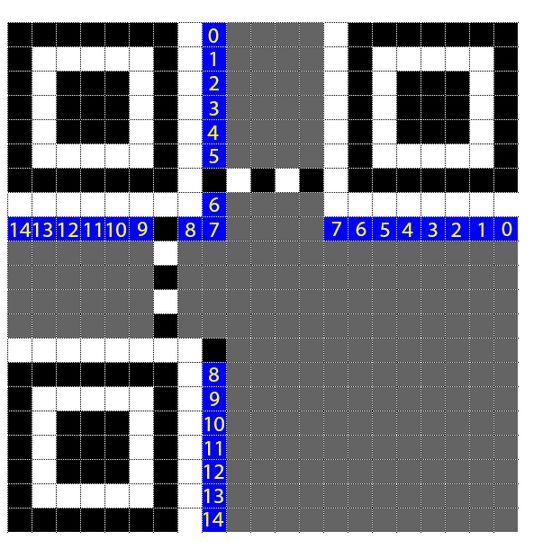
\includegraphics[width=0.5\textwidth]{figures/Formatinformation.jpg}
    \label{fig:2.10}
\end{figure}

The most significant bit of the stream will be placed in place number 14 and as a descending order the least significant bit will be placed in the place number 0.

Now the QR-Matrix is full and in other word the QR-code has been generated.

